\documentclass[oneside,a4paper,german,parskip=half,draft]{scrbook}

\usepackage[latin1]{inputenc}

%Neue Deutsche Rechtschreibung
\usepackage{ngerman}

%Seitenheader
\usepackage{fancyhdr}
\pagestyle{fancy}
\rhead{\nouppercase{\rightmark}}
\lhead{\nouppercase{\leftmark}}

%Standartfont
\usepackage[T1]{fontenc}
%\usepackage{fourier}
%\usepackage{libertine}

%Zusatzpaket f�r mathematische Ausdr�cke
\usepackage{amsmath}

%Zusatzfonts f�r mathbb usw.
\usepackage{amsfonts}
\usepackage{mathrsfs}

%Verbessertes Ref
\usepackage[german]{varioref}

%Links
\usepackage{hyperref}

%Stichwortverzeichnis
\usepackage{makeidx}
\makeindex

%Acronyme
\usepackage[nolist,nohyperlinks]{acronym}

%Anpassbare Enumerates/Itemizes
\usepackage{enumitem}

%Tikz/PGF Zeichnenpaket
\usepackage{pgf}
\usepackage{tikz}
\usetikzlibrary{mindmap,trees,decorations,decorations.pathreplacing,decorations.pathmorphing,calc,arrows,automata}

%F�r graphische Todos
\usepackage[colorinlistoftodos, obeyDraft]{todonotes}

%Paket zum Berechnen von Textbreiten und H�hen
\usepackage{calc}

%BibTeX
%\usepackage{cite}
%\usepackage{bibgerm}
%\bibliographystyle{gerplain}

%F�r das manipulieren von Captions in Figuren
\usepackage{caption}

%F�r das anpassen von theoremen
\usepackage{amsthm}

%F�r die farbigen Boxen
\usepackage{xcolor}
\usepackage{framed}

%Um die Seite in mehrere Spalten aufzuteilen
\usepackage{multicol}

%F�r zwischenr�ume in W�rtern
\usepackage{xspace}

%Quellcode Einbindung
\usepackage{listings}
\lstset{
basicstyle=\ttfamily
}

%F�r das durchstreichen von Bl�cken
\usepackage{cancel}

%F�r Commandos mit zwei opotionalen Argumenten
\usepackage{twoopt}

% \if\blank --- checks if parameter is blank (Spaces count as blank) 
% \if\given --- checks if parameter is not blank: like \if\blank{#1}\else 
% \if\nil --- checks if parameter is null (spaces are NOT null) 
% use \if\given{ } ... \else ... \fi etc. 
% Beispiel: \newcommand{\blah}[1]{\if\blank{#1}Leer\else#1\fi}
% 
{\catcode`\!=8 % funny catcode so ! will be a delimiter 
\catcode`\Q=3 % funny catcode so Q will be a delimiter 
\long\gdef\given#1{88\fi\Ifbl@nk#1QQQ\empty!} 
\long\gdef\blank#1{88\fi\Ifbl@nk#1QQ..!}% if null or spaces 
\long\gdef\nil#1{\IfN@Ught#1* {#1}!}% if null 
\long\gdef\IfN@Ught#1 #2!{\blank{#2}} 
\long\gdef\Ifbl@nk#1#2Q#3!{\ifx#3}% same as above 
}

%<Commandos>
%In geschweifte Klammern setzen
\newcommand{\gklamm}[1]{\ensuremath{\left\{#1\right\}}}

%In eckige Klammern setzen
\newcommand{\eklamm}[1]{\ensuremath{\left[#1\right]}}

%In runde Klammern setzen
\newcommand{\rklamm}[1]{\ensuremath{\left(#1\right)}}

%In Betragsstriche Setzen
\newcommand{\betrag}[1]{\ensuremath{\left|#1\right|}}

%Script zum Eingeben von l�ngeren Beispielen
\newcommand{\bsp}[3][]
{
\if\blank{#3}\textalign{\textbf{#2}}{#1}\else
\textbf{#2} #1
\par
\begingroup
\leftskip=1.28em
\setlist[1]{labelindent=1.28em, leftmargin=*}
#3
\par
\endgroup\fi
}

%Script um Text einzur�cken
\newcommand{\textalign}[2]{
\begin{minipage}[b]{\widthof{#1} + \widthof{\space}}
#1
\end{minipage}
\begin{minipage}[t]{\linewidth-\widthof{#1}-\widthof{\space}}
#2
\end{minipage}
}

%Script um Text einzur�cken ohne Ausgabe
\newcommand{\textfakealign}[3]{
\begin{minipage}[b]{\widthof{#1} + \widthof{\space}}
\if\blank{#2}$ $\else#2\fi
\end{minipage}
\begin{minipage}[t]{\linewidth-\widthof{#1}-\widthof{\space}}
#3
\end{minipage}
}

%Indexe
%Normaler Index
\newcommand{\indexn}[2][]{#2\if\blank{#1}\index{#2}\else\index{#1}\fi}
%Unterstrichener Index
\newcommand{\indexu}[2][]{\underline{#2}\if\blank{#1}\index{#2}\else\index{#1}\fi}
%Kursiver Index
\newcommand{\indexi}[2][]{\textit{#2}\if\blank{#1}\index{#2}\else\index{#1}\fi}
%Fetter Index
\newcommand{\indexb}[2][]{\textbf{#2}\if\blank{#1}\index{#2}\else\index{#1}\fi}

%Definitionen, Beispiele, S�tze
\newenvironment{fshaded}[2]{%
\def\FrameCommand{\fcolorbox{#1}{#2}}%
\MakeFramed {\FrameRestore}}%
{\endMakeFramed}

\theoremstyle{definition}
\newtheorem{definition}{\ac{Def.}}[part]
\newenvironment{fdefinition}[1][]{\definecolor{shadecolor_definition}{rgb}{.87,.94,.96}
\definecolor{framecolor_definition}{rgb}{0,0,0}%
\begin{fshaded}{framecolor_definition}{shadecolor_definition}\begin{definition}[#1]}{\end{definition}\end{fshaded}}

\newtheorem{satz}[definition]{Satz}
\newenvironment{fsatz}[1][]{\definecolor{shadecolor_satz}{rgb}{.87,.96,.56}
\definecolor{framecolor_satz}{rgb}{0,0,0}%
\begin{fshaded}{framecolor_satz}{shadecolor_satz}\begin{satz}[#1]}{\end{satz}\end{fshaded}}

\newtheorem{beweis}{Beweis}[part]
\newenvironment{fbeweis}[1][]{\definecolor{shadecolor_beweis}{rgb}{1.00,.96,.92}
\definecolor{framecolor_beweis}{rgb}{0,0,0}%
\begin{fshaded}{framecolor_beweis}{shadecolor_beweis}\begin{beweis}[#1]}{\end{beweis}\end{fshaded}}

\theoremstyle{remark}
\newtheorem{notation}{Notation}[part]
\newenvironment{fnotation}[1][]{\definecolor{shadecolor_notation}{rgb}{.90, .90, .90}
\definecolor{framecolor_notation}{rgb}{0,0,0}%
\begin{fshaded}{framecolor_notation}{shadecolor_notation}\begin{notation}[#1]}{\end{notation}\end{fshaded}}

\newtheoremstyle{note}% name
	{1em}			%Space above
	{1em}			%Space below
	{}				%Body font
	{}				%Indent amount (empty = no indent, \parindent = para indent)
	{\bfseries}	%Thm head font
	{:}			%Punctuation after thm head
	{.5em}		%Space after thm head: " " = normal interword space; \newline = linebreak
	{}				%Thm head spec (can be left empty, meaning `normal')

\newtheoremstyle{notelite}% name
	{3pt}			%Space above
	{3pt}			%Space below
	{}				%Body font
	{}				%Indent amount (empty = no indent, \parindent = para indent)
	{\itshape}	%Thm head font
	{:}			%Punctuation after thm head
	{.5em}		%Space after thm head: " " = normal interword space; \newline = linebreak
	{}				%Thm head spec (can be left empty, meaning `normal')

\theoremstyle{note}
\newtheorem*{beispiel}{Beispiel}

\theoremstyle{notelite}
\newtheorem*{anmerkung}{Anmerkung}
\newtheorem*{beobachtung}{Beobachtung}
\newtheorem*{bemerkung}{Bemerkung}
\newtheorem*{achtung}{Achtung}
%%%%%%%%Arabische in R�mische Zahl umwandeln
\newcommand{\RM}[1]{\ensuremath{\mbox{\MakeUppercase{\romannumeral #1}}}}
\newcommand{\rM}[1]{\ensuremath{\mbox{\romannumeral #1}}}
%</Commandos>

%<Abk�rzungen>
\newcommand{\Ra}{\ensuremath{\Rightarrow}}
\newcommand{\ra}{\ensuremath{\rightarrow}}
\newcommand{\La}{\ensuremath{\Leftarrow}}
\newcommand{\la}{\ensuremath{\leftarrow}}
\newcommand{\Ral}{\ensuremath{\Longrightarrow}}
\newcommand{\ral}{\ensuremath{\longrightarrow}}
\newcommand{\Lra}{\ensuremath{\Leftrightarrow}}
\newcommand{\lra}{\ensuremath{\leftrightarrow}}
\newcommand{\hra}{\ensuremath{\hookrightarrow}}
\newcommand{\mul}{\ensuremath{\cdot}}
\newcommand{\grgl}{\ensuremath{\geq}}
\newcommand{\klgl}{\ensuremath{\leq}}
\newcommand{\oder}{\ensuremath{\vee}}
\newcommand{\und}{\ensuremath{\wedge}}
\newcommand{\mal}{\ensuremath{\cdot}}
\newcommand{\matrixp}[1]{\ensuremath{\begin{pmatrix} #1 \end{pmatrix}}}
\newcommand{\coloneqq}{\mathrel{\mathop:\!\!=}}
\newcommand{\ceq}{\ensuremath{\coloneqq}}
\newcommand{\tx}[1]{\ensuremath{\text{#1}}}
\newcommand{\rkl}[1]{\ensuremath{\rklamm{#1}}}
\newcommand{\N}{\ensuremath{\mb{N}}}
\newcommand{\R}{\ensuremath{\mb{R}}}
\newcommand{\Z}{\ensuremath{\mb{Z}}}
\newcommand{\stack}[2]{\ensuremath{\stackrel{#1}{#2}}}
\newcommand{\ub}[2]{\ensuremath{\underbrace{#1}_{#2}}}

%Todo, Insert, Mark, Img
\newcommand{\Todo}[1]{\todo[inline]{TODO: #1}}
\newcommand{\Insert}[1]{\todo[inline, color=green!40]{INSERT: #1}}
\newcommand{\Mark}[1]{\todo[inline, nolist, color=blue!40]{MARK: #1}}
\newcommand{\Img}[1]{\todo[inline, nolist, color=black!40]{IMG: #1}}

%Sin, Cos, Tan, Dim, Span, Arccos, Limes
\DeclareMathOperator{\spano}{span}
\DeclareMathOperator{\lb}{lb}

\newcommand{\sinx}[1]{\ensuremath{\sin{\left(#1\right)}}}
\newcommand{\cosx}[1]{\ensuremath{\cos{\left(#1\right)}}}
\newcommand{\tanx}[1]{\ensuremath{\tan{\left(#1\right)}}}
\newcommand{\dimx}[1]{\ensuremath{\dim{\left(#1\right)}}}
\newcommand{\spanx}[1]{\ensuremath{\spano{\left(#1\right)}}}
\newcommand{\arccosx}[1]{\ensuremath{\arccos{\left(#1\right)}}}

%Schriften
\newcommand{\mb}[1]{\ensuremath{\mathbb{#1}}}
%</Abk�rzungen>




%<Einstellung f�r Hyperref>%%%%%%%%%%%%%%%%%%%%%%%%%%%%%%%%%%%%%%%%%%%%%%%%%%%%
\hypersetup{colorlinks=false, linkcolor=black, breaklinks=true, bookmarksdepth=3,unicode=false,bookmarksnumbered=true,
pdftitle={L�sung f�r 1. �bung der Grundlagen Informatik SS2009},
pdfauthor={Thaller Alexander},
pdfsubject={L�sung f�r 1. �bung der Grundlagen Informatik SS2009},pdfkeywords={l�sung,studium,�bung}}
%</Einstellung f�r Hyperref>%%%%%%%%%%%%%%%%%%%%%%%%%%%%%%%%%%%%%%%%%%%%%%%%%%%

\begin{document}
\begin{acronym}
	\acro{acr}{Akronym}
	\acro{zB}[\ensuremath{\mbox{z.\,B.}\xspace}]{zum Beispiel}
	\acro{bel.}{beliebigem}
	\acro{Def.}{Definition}
	\acro{gdw.}[\ensuremath{\mbox{g.\,d.\,w.}\xspace}]{genau dann wenn}
	\acro{def.}{definiert}
	\acro{Opt.}{Optimiert}
	\acro{DEA}{Deterministischer endlicher Automat}
	\acro{akzept.}{akzeptierende}
	\acro{bzw.}{beziehungsweise}
	\acro{bzgl.}{bez�glich}
	\acro{NEA}{Nichtdeterministische endliche Automaten}
	\acro{Ber.}{Berechnung}
	\acro{Berechn.}{Berechnung}
	\acro{Bew.}{Beweis}
	\acro{d.h}[\ensuremath{\mbox{d.\,h.}\xspace}]{daher}
	\acro{akz.}{akzeptierende}
	\acro{ex.}{existiert}
	\acro{Anw.}{Anwendung}
	\acro{M�gl.}{M�glichkeit}
\end{acronym}

%\maketitle
\setcounter{tocdepth}{0}
\setcounter{secnumdepth}{-1}
\addtocounter{chapter}{2}
%\tableofcontents
%\newpage
%<Text>%%%%%%%%%%%%%%%%%%%%%%%%%%%%%%%%%%%%%%%%%%%%%%%%%%%%%%%%%%%%%%%%%%%%%%%%
%\chapter*{1. �bung}
\section*{1. Aufgabe}
$\Sigma = \gklamm{0, 1}$, $L_1 = \gklamm{0, 00, 000}$, $L_2 = \gklamm{0, 1, 01}$
\begin{enumerate}[label=(\alph*)]
\item $L_1 \mal L_2 = \gklamm{00, 01, 001, 000, 0001, 0000, 00001}$
\item $L_1^3 = \gklamm{0^3, 0^4, 0^5, 0^6, 0^7, 0^8, 0^9}$
\item $L_1^{\mathcal{C}} = \Sigma^* - L_1$
\item $L_1^* = \gklamm{\epsilon, 0, 00, 000, 0^4, \dots}$
\item $\emptyset^* = \gklamm{\epsilon}$
\end{enumerate}

\section*{2. Aufgabe}
\begin{enumerate}[label=(\alph*)]
\item $\del$
		\begin{itemize}
		\item $\del(\epsilon) = \epsilon$
		\item sei $w = av$, falls $a = b$ wobei $b$ der zu l�schende Buchstabe ist, sei $\del(w) = del(v)$. Ansonsten ist $\del(w) = a \del(v)$.
		\end{itemize}

\item $\gicount$
		\begin{itemize}
		\item $\gicount(\epsilon) = 0$
		\item sei $w = av$, falls $a = b$ wobei $b$ der zu z�hlende Buchstabe sei ist $\gicount(w) = \gicount(v) + 1$. Ansonsten ist $\gicount(w) = \gicount(v) + 0$.
		\end{itemize}
\end{enumerate}

\section*{3. Aufgabe}
$\Sigma = \gklamm{0, 1, \sharp}$
\begin{enumerate}[label=(\alph*)]
\item Die Anzahl der verschiedenen W�rter ist die Anzahl der Zeichen in $\Sigma$ hoch $n$ wobei $n$ die Anzahl der Stellen ist. In dem Fall $\Sigma = \gklamm{0, 1, \sharp}$ ist die Anzahl also $n^3$.
\item Es gibt $\matrixp{n\\k}$ M�glichkeiten das Symbol zu platzieren. F�r jede Platzierung hat man eine M�glichkeit weniger ein also $(n - k)$. Daraus ergibt sich die Formel:
		\[\matrixp{n\\k} \mal 2^{(n - k)}\]

\item Die Antwort ergibt sich aus der vorherigen L�sung nur muss man alle einzelnen Wahrscheinlichkeiten des Zeichens aufsummieren. Es folgt also:
		\[\sum_{i = k}^n \matrixp{n\\i} \mal 2^{n - i}\]
\end{enumerate}

\section*{4. Aufgabe}
$\Sigma_{\text{Bool}} = \gklamm{0, 1}$, $\underbrace{\rklamm{L_1 \cup L_2}^*}_{M_1} 0 \underbrace{L_1^* \cup L_2^*}_{M_2}$
\subsection*{Beispielsprachen}
$L_1 = \gklamm{01}$\\
$L_2 = \gklamm{10}$

\subsection*{Beweis der Aussage}
\subsubsection*{Annahme}
$M_1 \subseteq M_2 \wedge M_2 \subseteq M_1$\\
\Ra $L_1^* \subseteq \rklamm{L_1 \cup L_2}^* \wedge L_2^* \subseteq \rklamm{L_1 \cup L_2}^*$

\subsubsection*{Beweis}
\begin{enumerate}
\item $M_1 \subseteq M_2$
		\begin{align*}
		u &\in \rklamm{L_1 \cup L_2}^*\\
		u &\in \rklamm{\gklamm{01} \cup \gklamm{10}}^*\\
		u &= \gklamm{01}\\
		&\Ra u \in \rklamm{\gklamm{01} \cup \gklamm{10}}^* \text{ da } \gklamm{01} \in \gklamm{01}^*
		\end{align*}
		\Ra $u \in M_1$
\item $M_2 \subseteq M_1$
		\begin{align*}
		u &\in L_1^* \cup L_2^*\\
		u &\in \gklamm{01}^* \cup \gklamm{10}^*\\
		u &= \gklamm{01}\\
		&\Ra u \in \gklamm{01}^* \cup \gklamm{10}^* \text{ da } \gklamm{01} \in \gklamm{01}^*
		\end{align*}
		\Ra $u \in M_1$
\end{enumerate}
\Ra $u \in M_1 \wedge M_2$ \Ra $M_1 = M_2$
\begin{flushright}$\blacksquare$\end{flushright}
\label{TotalPages}

\chapter{2. �bung}
\section{1. Aufgabe (2+2 Punkte)}
\begin{enumerate}[label=(\alph*)]
\item Man kann den Graphen \vref{fig:Uebung_GraphA1} in Form einer Adjazentenmatrix (Abbildung \vref{fig:Uebung_A1}) schreiben welche die Aussage enth�lt ($0$ ist nicht verbunden, $1$ ist verbunden) ob zwei Knoten �ber eine Kante miteinander verbunden sind.
		\begin{figure}[htb]
		\centering
		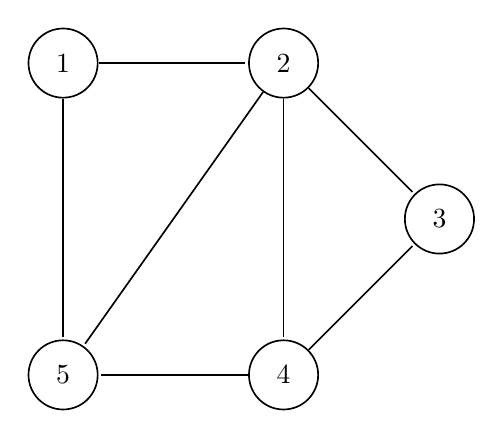
\begin{tikzpicture}[->,>=stealth',shorten >=1pt,auto,node distance=2.8cm,semithick]
		\node[state] (n3) {3};
		\node[state] (n2) [above left of=n3] {2};
		\node[state] (n4) [below left of=n3] {4};
		\node[state] (n1) [left of=n2] {1};
		\node[state] (n5) [left of=n4] {5};

		\path[-] (n1) edge (n2);
		\path[-] (n1) edge (n5);
		
		\path[-] (n2) edge (n5);
		\path[-] (n2) edge (n3);
		\path[-] (n2) edge (n4);
		
		\path[-] (n4) edge (n5);
		\path[-] (n4) edge (n3);
		\end{tikzpicture}
		\captionsetup{labelformat=simplegraph}
		\caption{}
		\label{fig:Uebung_GraphA1}
		\end{figure}
		wird zu
		\begin{figure}[htb]
		\centering
		\[\begin{array}{c|ccccc}
		 &1&2&3&4&5\\
		\hline
		1&0&1&0&0&1\\
		2&1&0&1&1&1\\
		3&0&1&0&1&0\\
		4&0&1&1&0&1\\
		5&1&1&0&1&0
		\end{array}\]
		\caption{}
		\label{fig:Uebung_A1}
		\end{figure}

\item $w = 110 110 111 100 101 111$\\
		Alte Darstellung: $11\sharp 01\sharp 10\sharp 11\sharp 11\sharp 00\sharp 10\sharp 11\sharp 11$ (26 Zeichen)\\
		Neue Darstellung: $110\sharp 110\sharp 111\sharp 100\sharp 101\sharp 111$ (23 Zeichen)
\end{enumerate}

\section{2. Aufgabe (8+2 Punkte)}
\begin{enumerate}[label=(\alph*)]
\item $\gklamm{a}^* \gklamm{b}^* = \gklamm{a^i b^j \vert i, j \in \N}$
		\begin{align*}
		&x \in \gklamm{a}^*\gklamm{b}^*\\
		&x = y z (y \in \gklamm{a}^*, z \in \gklamm{b}^*)\\
		\Ra& y \in \gklamm{a}^k, z \in \gklamm{b}^m \tx{ f�r } \exists k, m \in \N\\
		\Ra& x = a^k b^m\\
		\Ra& x \in \gklamm{a^i b^j \vert i, j \in \N}
		\end{align*}
		\Ra $x \in \gklamm{a}^* \gklamm{b}^* \und x \in \gklamm{a^i b^j \vert i, j \in \N}$\\
		\Ra Die Aussage ist wahr

\item $\rklamm{\gklamm{a}^* \gklamm{b}^*}^* = \rklamm{\gklamm{a, b}^2}^*$\\
		$a = 0$, $b = 1$\\
		\begin{align*}
		\rklamm{\gklamm{a}^* \gklamm{b}^*}^* &= \rklamm{\gklamm{\epsilon, 0, 00, 000, \dots} \gklamm{\epsilon, 1, 11, 111, \dots}}^*\\
		&=\rklamm{\gklamm{\epsilon, 1, 11, 111, 0, 01, 011, 0111, 001, 0011, 00111, \dots}}^*\\
		&=\gklamm{\epsilon, 1, 11, 111, 0, 00, 000, 11, 1111, 111111, \dots}\\
		\rklamm{\gklamm{a, b}^2}^* &= \rklamm{\gklamm{01} \gklamm{01}}^*\\
		&= \rklamm{\gklamm{0101}}^*\\
		&= \gklamm{\epsilon, 0101, 01010101, \dots}
		\end{align*}
		\Ra $1 \in \rklamm{\gklamm{a}^* \gklamm{b}^*}^* \und 1 \notin \rklamm{\gklamm{a, b}^2}^*$\\
		\Ra Die Aussage ist falsch
\end{enumerate}

\section{3. Aufgabe (6+4+4 Punkte)}
\begin{enumerate}[label=(\alph*)]
\item $L_2 = \gklamm{w \in \Sigma_{\tx{Bool}}^* \vert \betrag{w}_0 = 4}$ - alle Bin�rw�rter, die exakt 4 Nullen enthalten.\\
		L�sung siehe Abbildung \vref{fig:Uebung2_3a}.
		\begin{figure}[hbt]
		\centering
		\begin{tikzpicture}[->,>=stealth',shorten >=1pt,auto,node distance=2.8cm,semithick]
		\node[state,initial,initial text=] (n1) {};
		\node[state] (n2) [right of=n1] {};
		\node[state] (n3) [right of=n2] {};
		\node[state] (n4) [right of=n3] {};
		\node[state,accepting] (n5) [right of=n4] {};
		\node[state] (n6) [below of=n5] {DS};
		
		\path[->] (n1) edge[loop above] node[right] {$1$} ();
		\path[->] (n2) edge[loop above] node[right] {$1$} ();
		\path[->] (n3) edge[loop above] node[right] {$1$} ();
		\path[->] (n4) edge[loop above] node[right] {$1$} ();
		\path[->] (n5) edge[loop above] node[right] {$1$} ();
		\path[->] (n6) edge[loop below] node[right] {$1, 0$} ();
		
		\path[->] (n1) edge node[above] {$0$} (n2);
		\path[->] (n2) edge node[above] {$0$} (n3);
		\path[->] (n3) edge node[above] {$0$} (n4);
		\path[->] (n4) edge node[above] {$0$} (n5);
		\path[->] (n5) edge node[right] {$0$} (n6);
		\end{tikzpicture}
		\caption{L�sung f�r 3. Aufgabe (a)}
		\label{fig:Uebung2_3a}
		\end{figure}

\item $L_3 = \gklamm{w \in \Sigma_{\tx{Bool}}^* \vert 110 \tx{ ist kein Teilwort von } w}$
		L�sung siehe Abbildung \vref{fig:Uebung2_3b}.
		\begin{figure}[hbt]
		\centering
		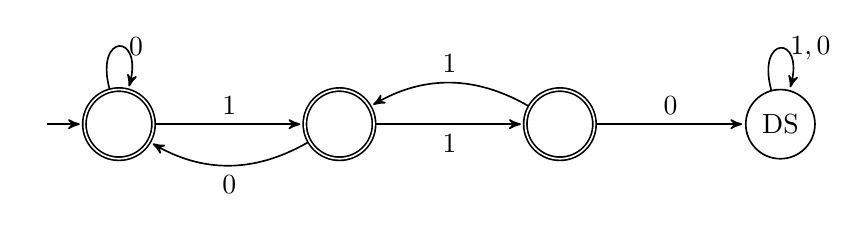
\begin{tikzpicture}[->,>=stealth',shorten >=1pt,auto,node distance=2.8cm,semithick]
		\node[state,initial,initial text=,accepting] (n1) {};
		\node[state,accepting] (n2) [right of=n1] {};
		\node[state,accepting] (n3) [right of=n2] {};
		\node[state] (n4) [right of=n3] {DS};

		\path[->] (n1) edge[loop above] node[right] {$0$} ();
		\path[->] (n4) edge[loop above] node[right] {$1, 0$} ();

		\path[->] (n1) edge node[above] {$1$} (n2);
		\path[->] (n2) edge node[below] {$1$} (n3);
		\path[->] (n3) edge node[above] {$0$} (n4);

		\path[->] (n2) edge [bend left] node[below] {$0$} (n1);
		\path[->] (n3) edge [bend right] node [above] {$1$} (n2);
		\end{tikzpicture}
		\caption{L�sung f�r 3. Aufgabe (b)}
		\label{fig:Uebung2_3b}
		\end{figure}

\item $L_4 = \gklamm{w \in \Sigma_{\tx{Bool}}^* \vert \betrag{w} \klgl 5}$
		L�sung siehe Abbildung \vref{fig:Uebung2_3c}.
		\begin{figure}[hbt]
		\centering
		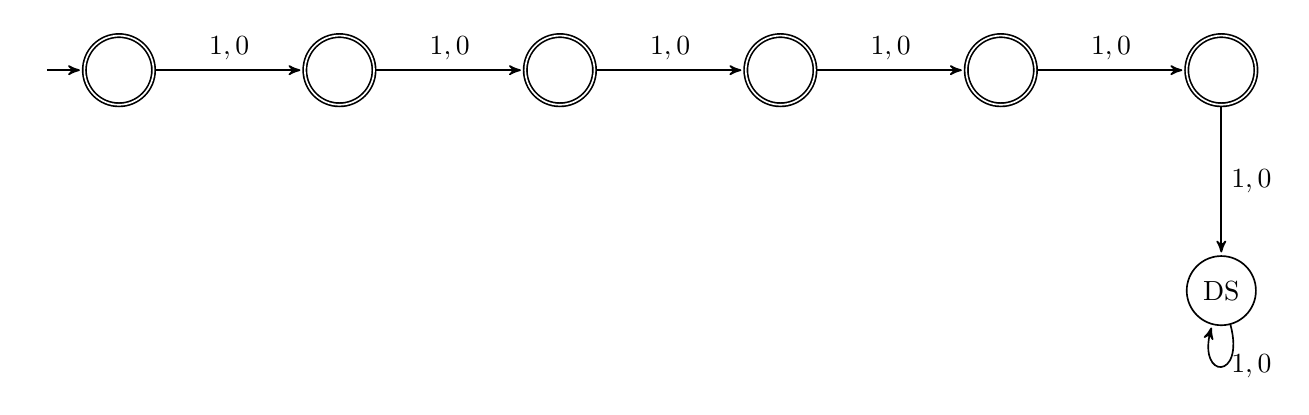
\begin{tikzpicture}[->,>=stealth',shorten >=1pt,auto,node distance=2.8cm,semithick]
		\node[state,initial,initial text=,accepting] (n1) {};
		\node[state,accepting] (n2) [right of=n1] {};
		\node[state,accepting] (n3) [right of=n2] {};
		\node[state,accepting] (n4) [right of=n3] {};
		\node[state,accepting] (n5) [right of=n4] {};
		\node[state,accepting] (n6) [right of=n5] {};
		\node[state] (n7) [below of=n6] {DS};

		\path[->] (n7) edge [loop below] node[right] {$1,0$} ();
		\path[->] (n1) edge node[above] {$1, 0$} (n2);
		\path[->] (n2) edge node[above] {$1, 0$} (n3);
		\path[->] (n3) edge node[above] {$1, 0$} (n4);
		\path[->] (n4) edge node[above] {$1, 0$} (n5);
		\path[->] (n5) edge node[above] {$1, 0$} (n6);
		\path[->] (n6) edge node[right] {$1, 0$} (n7);
		\end{tikzpicture}
		\caption{L�sung f�r 3. Aufgabe (c)}
		\label{fig:Uebung2_3c}
		\end{figure}
\end{enumerate}

\section{4. Aufgabe (3 Punkte)}
\[\left.
\begin{array}{lll}
h(0) &=& 000\\
h(1) &=& 001\\
h(x) &=& 010\\
h('(') &=& 011\\
h(')') &=& 100\\
h(\vee) &=& 101\\
h(\wedge) &=& 110\\
h(\neg) &=& 111\\
\end{array}\right\} h: \Sigma_{\tx{logic}}^* \ra \Sigma_{\tx{Bool}}^*
\]

%\section{5. Aufgabe (10 Zusatzpunkte)}

%</Text>%%%%%%%%%%%%%%%%%%%%%%%%%%%%%%%%%%%%%%%%%%%%%%%%%%%%%%%%%%%%%%%%%%%%%%%

%Literaturverzeichnis
\newpage
\addcontentsline{toc}{part}{Literaturverzeichnis}
\bibliography{literatur}{}

%Stichwortverzeichnis
\newpage
\renewcommand{\indexname}{Stichwortverzeichnis}
\addcontentsline{toc}{part}{Stichwortverzeichnis}
\printindex

\end{document}


